\chapter{Triggers}

\section{Trigger Properties}

The \menustyle{Setup / Trigger} menu opens the trigger properties dialog (Fig. \ref{trigger-properties}).

The Trigger Type box allows the type of trigger to be chosen. The list of available triggers depends on the instrument
model and installed software options.

The Trigger Offset field specifies the time from the \emph{start} of the waveform to the trigger point. Positive values
move the trigger later into the waveform, negative values introduce a delay between the trigger and the start of the
waveform. \footnote{This is a different convention than most oscilloscopes, which measure the trigger position from the
\emph{midpoint} of the waveform. Since glscopeclient decouples the acquisition length from the UI zoom setting,
measuring from the midpoint makes little sense as there are no obvious visual cues to the midpoint's location.}

\begin{figure}[h]
\centering
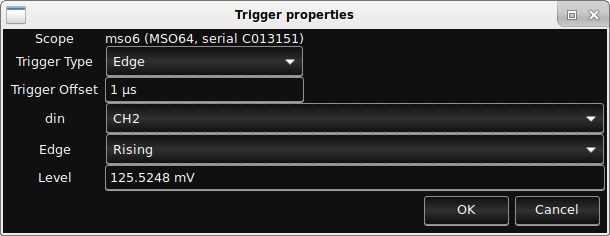
\includegraphics[width=9cm]{images/trigger-properties.png}
\caption{Trigger properties dialog}
\label{trigger-properties}
\end{figure}

The remaining settings in the trigger properties dialog depend on the specific trigger type chosen.

\section{Dropout}

Triggers when a signal stops toggling for a specified amount of time.

\section{Edge}

Triggers on edges in the signal.

\section{Pulse Width}

Triggers when a high or low pulse meeting specified width criteria is seen.

\section{Runt}

Triggers when a pulse crosses one threshold, but not a second.

\section{Slew Rate}

Triggers when an edge is faster or slower than a specified rate.

\section{UART}

Triggers when a byte or byte sequence is seen on a UART.

\section{Window}

Triggers when a signal goes above or below specified thresholds.
